\section*{Синтез и построение одноразрадяного сумматора}
\addcontentsline{toc}{section}{Синтез и построение одноразрядного сумматора}
\subsection*{Построение одноразрядного сумматора}
\addcontentsline{toc}{subsection}{Построение одноразрядного сумматора}

Для синтеза модели одноразрядного сумматора необходимо составить аналитическую модель 
посредством построения СДНФ для управляющих сигналов S и P из таблицы \ref{table:2}. \par

\begin{table}[h!]
    \begin{center}
        \begin{tabular}{ | m{1cm} | m{1cm} | m{1cm} | m{1cm} | m{1cm} | }
            \hline
            X & Y & Z & S & P \\ \hline
            0 & 0 & 0 & 0 & 0 \\ \hline 
            0 & 0 & 1 & 1 & 0 \\ \hline
            0 & 1 & 0 & 1 & 0 \\ \hline
            0 & 1 & 1 & 0 & 1 \\ \hline
            1 & 0 & 0 & 1 & 0 \\ \hline
            1 & 0 & 1 & 0 & 1 \\ \hline
            1 & 1 & 0 & 0 & 1 \\ \hline
            1 & 1 & 1 & 1 & 1 \\ \hline
        \end{tabular}
        \caption{Таблицы истинности одноразрядного сумматора}
        \label{table:2}
    \end{center}    
\end{table}

В результате составление СДНФ и ее упрощения получаем функции 
управляющих сигналов: \par

\begin{itemize}
    \item $S=Z(\overline{X}\overline{Y} \cup XY) \cup \overline{Z}(\overline{X}Y \cup X\overline{Y})$
    \item $P=Z(\overline{X}Y \cup X\overline{Y}) \cup XY$
\end{itemize}

На основании полученных функций построим модель одноразрадяного сумматора (рис. \ref{image:3}).

\begin{figure}[h]
    \centering
    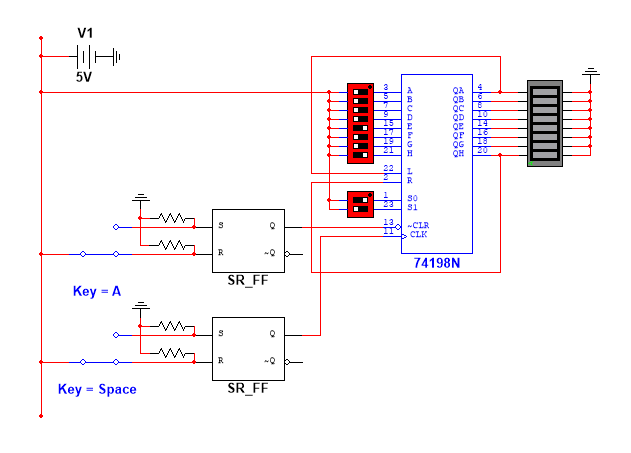
\includegraphics[scale=0.8]{image-3.png}
    \caption{Модель одноразрядного сумматора}
    \label{image:3}
\end{figure}

\newpage
\subsection*{Тестирование одноразрядного сумматора}
\addcontentsline{toc}{subsection}{Тестирование одноразрадяного сумматора}

Рассмотрим набор входящих сигналов $X=1,Y=0,Z=1$. Ожидаемые значения управляющих сигналов $S=0,P=1$.\par

\begin{figure}[h]
    \centering
    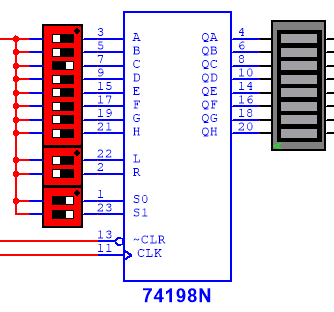
\includegraphics[scale=0.8]{image-4.png}
    \caption{Тестирование одноразрадяного сумматора}
    \label{image:4}
\end{figure}

Результат соответсвует ожиданию. Аналогино были протестированы остальные наборы входных сигналов.